\section{Results \& Analysis (cont.)}
% GOAL: Token/turn/retry analysis, failure taxonomy, cost-performance frontier.
% COMPRESSED to fit within 9-page body limit.

\subsection{Cost-Performance Frontier}

Figure~\ref{fig:cost_frontier} plots total elapsed time against pipeline score for all evaluated configurations.
Two patterns emerge:
(1)~\emph{high-score configurations are not always low-cost}---deepseek-reasoner achieves PL=63.5 but requires 15,987 seconds and 252 build attempts, while qwen3.6-flash achieves PL=98.6 in only 1,421 seconds with 52 builds;
(2)~\emph{cost efficiency varies dramatically}---the same pipeline score of 63.5 is achieved by three models with elapsed times ranging from 1,909s to 15,987s (an 8x difference).

\textbf{Process cost does not predict outcome.}
A linear regression of build count against pipeline score yields $R^2 = 0.003$ ($p = 0.82$); elapsed time against pipeline score yields $R^2 < 0.001$ ($p = 0.98$).
The combined model explains only 0.7\% of score variance.
This \emph{decoupling} is itself a diagnostic finding: agents that invest more computational budget (time, builds, retries) do not systematically achieve better outcomes.
The relationship is not monotonic---some agents achieve high scores with minimal effort (efficient solvers), while others exhaust their budget without progress (process collapse).
This demonstrates that process metrics capture \emph{qualitatively distinct} information from outcome metrics---not because they predict scores, but because they reveal \emph{how} agents arrive at their outcomes.
Two agents with identical pipeline scores may have radically different process profiles (efficient solver vs.\ persistent searcher), and this distinction is invisible to outcome-only evaluation but critical for deployment decisions (cost budgeting, timeout setting, scaffold optimization).
Process metrics thus serve a \emph{diagnostic} rather than \emph{predictive} role: they do not explain \emph{why} an agent succeeds, but they reveal \emph{how} it attempts to succeed, enabling targeted intervention when the process profile indicates inefficiency or collapse.

\begin{figure}[t]
\centering
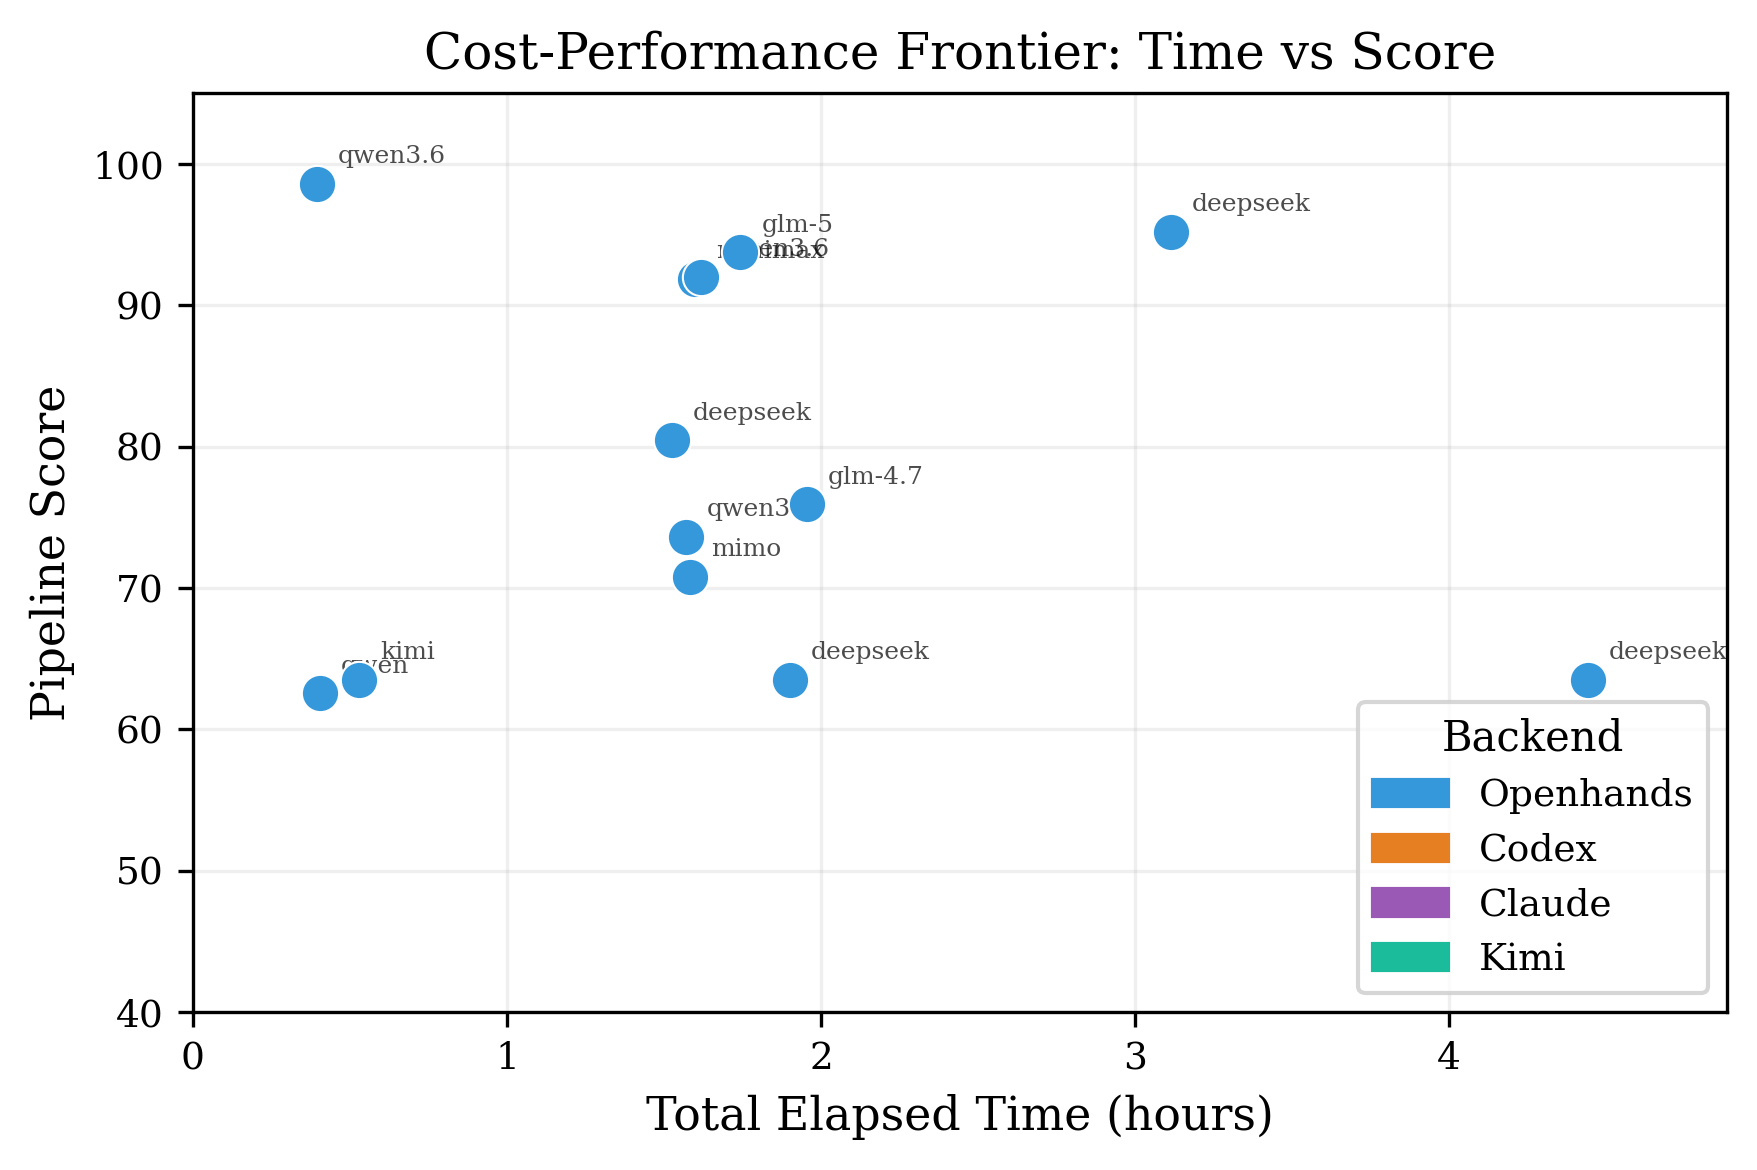
\includegraphics[width=\linewidth]{figures/fig_cost_performance.png}
\caption{Cost-performance frontier: elapsed time vs.\ pipeline score. The Pareto frontier highlights configurations achieving the best performance per unit time. The 8x cost difference between similarly-scoring agents (kimi-k2-thinking at 1,909s vs.\ deepseek-reasoner at 15,987s, both PL$\approx$63.5) demonstrates that outcome-only evaluation misses critical deployment information.}
\label{fig:cost_frontier}
\end{figure}

Build attempt counts reveal distinct agent behaviors: \emph{efficient solvers} (GPT-5.5: 80 builds, qwen3.6-flash: 52 builds) achieve high scores with minimal retries; \emph{persistent searchers} (deepseek-v4-flash: 181 builds, deepseek-reasoner: 252 builds) achieve moderate scores through exhaustive search; and \emph{collapsed agents} exhaust builds without progress. Agents that repeatedly build without modifying code exhibit \emph{process collapse}---a failure mode where the action loop decouples from productive problem-solving.

\subsection{Failure Taxonomy}

We categorize agent failures into five types: (1)~\emph{predecessor failure} (downstream unreachable), (2)~\emph{task-local reasoning failure} (cannot solve despite correct prerequisites), (3)~\emph{execution failure} (build/dependency errors), (4)~\emph{process collapse} (max-turn exhaustion, search loops), and (5)~\emph{cost overrun} (budget exhausted).

\begin{figure}[t]
\centering
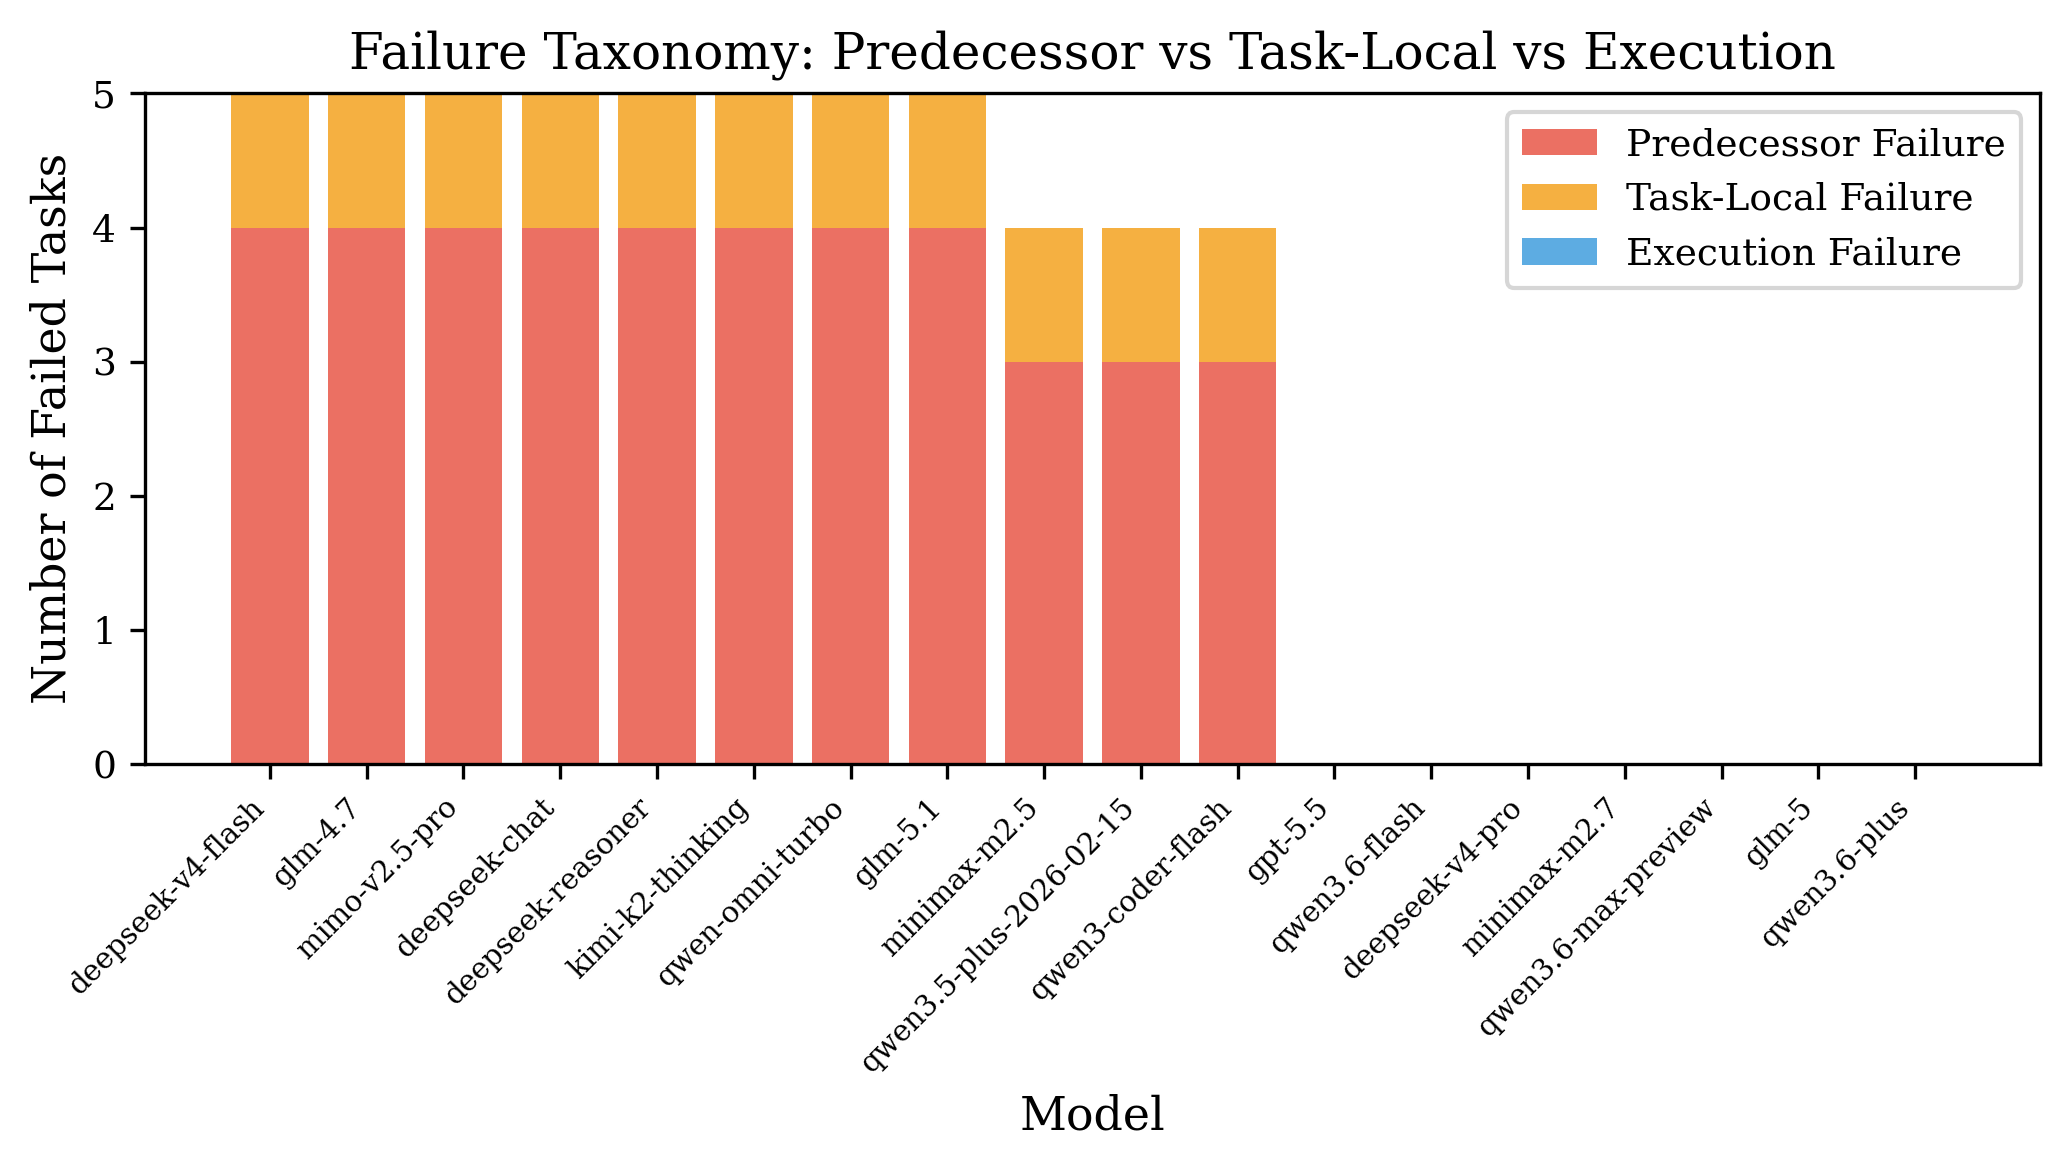
\includegraphics[width=\linewidth]{figures/fig_failure_taxonomy.png}
\caption{Failure taxonomy composition. Predecessor failure dominates without resurrection but is largely eliminated by resurrection, revealing the underlying task-local and execution failure distribution.}
\label{fig:failure_taxonomy}
\end{figure}

Figure~\ref{fig:failure_taxonomy} shows that predecessor failure dominates in the no-resurrection setting but is largely eliminated by resurrection, revealing the underlying distribution of task-local and execution failures. Process collapse is more prevalent in framework-based agents with unlimited iteration budgets, suggesting that scaffold design affects not just \emph{whether} the agent succeeds, but \emph{how} it fails.